section{3. Results}?

?\subsection{3.1  Key Observations}?

?\textbf{Persistence of Quantum Coherence}: Simulations revealed that microtubules ?
maintain coherence over extended durations, even under external decoherence ?
influences. This challenges assumptions of rapid decoherence in biological systems and ?
supports the hypothesis of intrinsic quantum stabilization mechanisms.?

?\textbf{Fibonacci Scaling as a Stabilizing Factor}: Incorporating Fibonacci scaling into the ?
models demonstrated resonance patterns that reduce wave packet dispersion and ?
conserve coherence, suggesting a fundamental role for universal mathematical principles ?
in biological quantum systems.?

?\textbf{Event Horizon Analogies}: Cytokine-induced decoherence simulations revealed ?
localized boundary-like behaviors analogous to astrophysical event horizons, suggesting ?
that microtubules may possess quantum boundaries that protect coherence.?


?\subsection{3.2  Visualization of Quantum Event Horizon-like Boundaries}?
?\begin{figure}[H]?
?\centering
?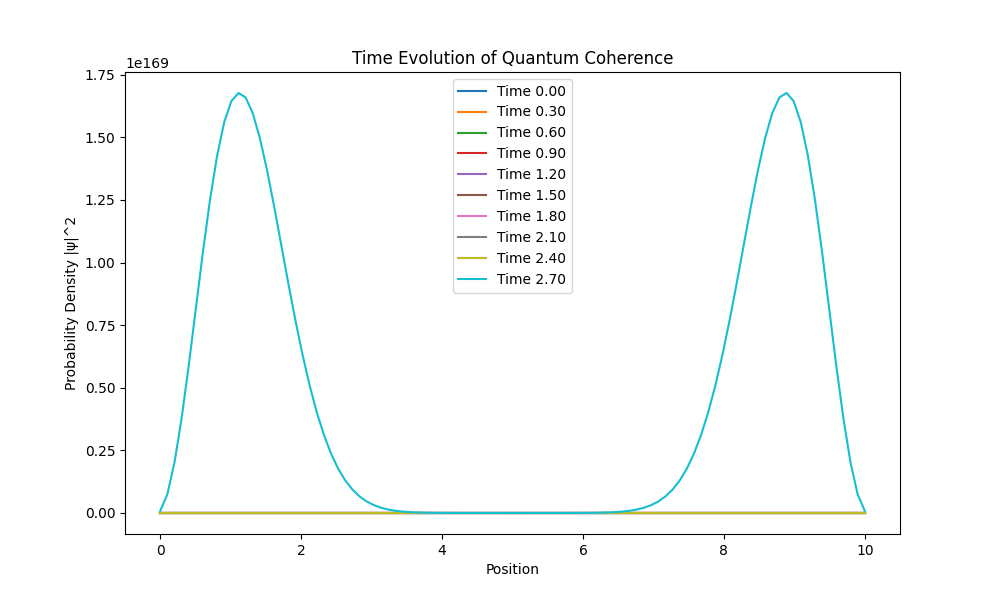
\includegraphics[width=0.8\textwidth]{figures/coherence_evolution_plot.png}?
?\caption{1D Simulation of Gaussian Wave Packet Dynamics:?
	?¥?	Visualization of coherence dynamics over time. Persistent peaks at ?
boundaries represent event horizon-like quantum sanctuaries.}?
?\label{fig 1:1D Simulation of Gaussian Wave Packet Dynamics}?
?\end{figure}?

?\subsection{3.3  Fibonacci Scaling}?
?\begin{figure}[H]?
?\centering
?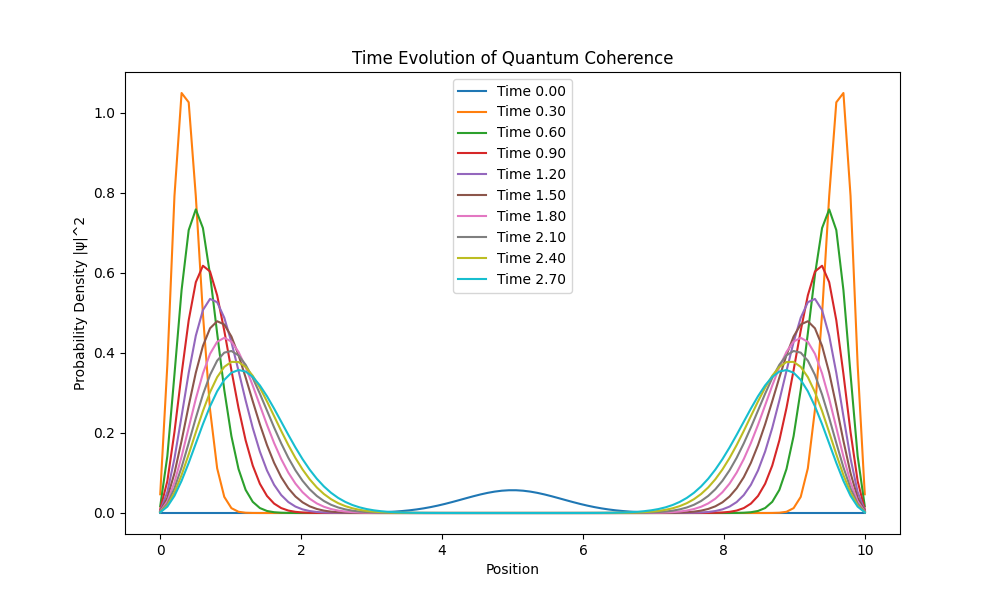
\includegraphics[width=0.8\textwidth]{figures/fibonacci_wavefunction_evolution.png}?
?\caption{Plot of time-evolved probability density (?) showing stabilization of coherence ?
under Fibonacci scaling principles.}?
?\label{fig 2:fibonacci_scaling}?
?\end{figure}?

?\subsection{3.4  2D Quantum Sanctuaries in Cylindrical Geometry}[H]?
?\begin{figure}[H]?
?\centering
?\includegraphics[width=0.8\textwidth]{figures/Cyndrical_time_evo0.png}?
?\includegraphics[width=0.8\textwidth]{figures/cylindrical_evo1.png}?
?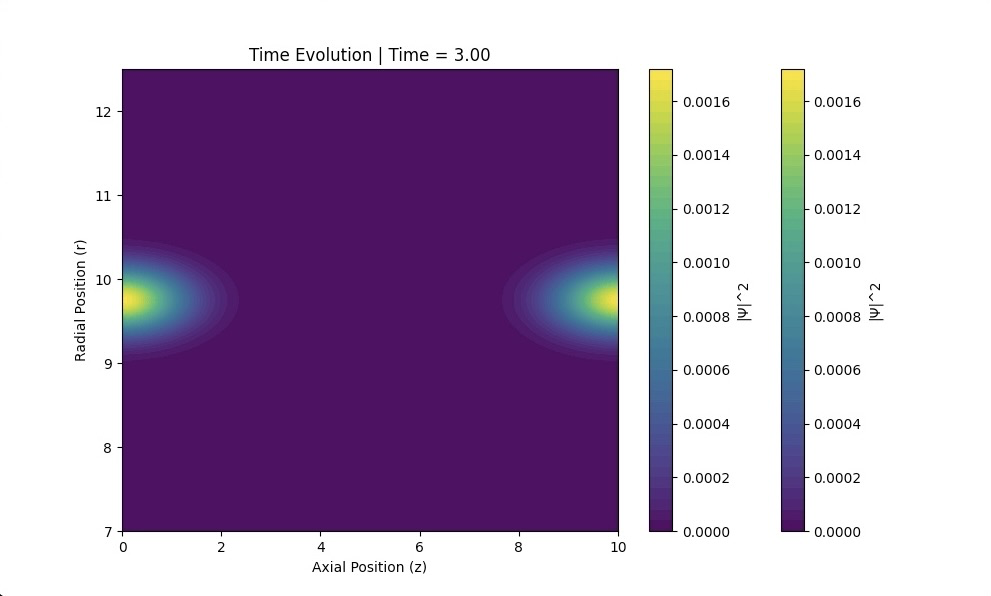
\includegraphics[width=0.8\textwidth]{figures/cylindrical_evo3.png}?
?\caption{Simulation of wavefunction probability density within a 2D cylindrical microtubule ?
model. Bright regions (yellow) indicate persistent coherence zones confined by event ?
horizon-like boundaries.}?
?\label{fig 3:Cylindrical_event_horizon}?
?\end{figure}?

?\subsection{3.5  2D Visualization of Wavefunction Probability Density in Cylindrical ?
Geometry
?\begin{figure}[H]?
?\centering
?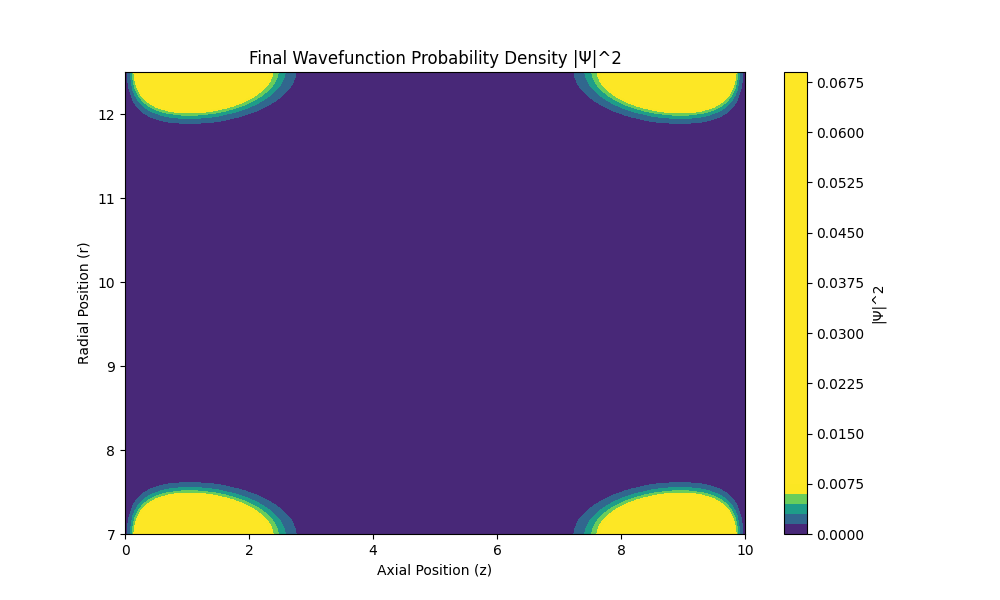
\includegraphics[width=0.8\textwidth]{figures/wavefunction_probability_density.png}?
?\caption{2D Quantum Sanctuaries in Cylindrical Geometry:?
Simulation of wavefunction probability density within a 2D cylindrical microtubule model. ?
Bright regions (yellow) indicate persistent coherence zones confined by event horizon-like ?
boundaries.}?
?\label{fig:Cylindrical_PD_EVHB}?
?\end{figure}?

?\begin{figure}[H]?
?\centering
?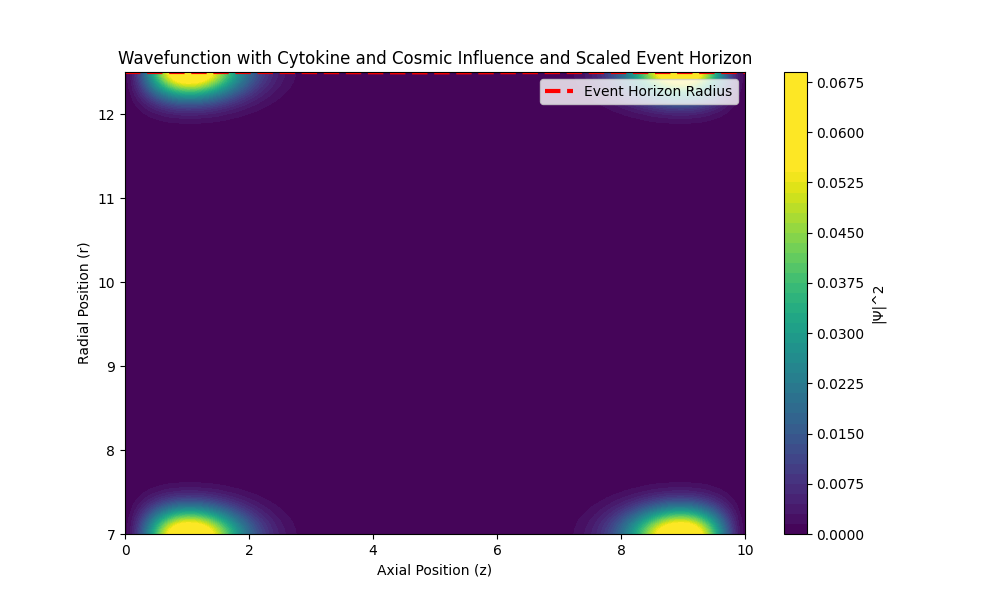
\includegraphics[width=0.8\textwidth]{figures/wavefunction_event_horizon_plot.png}?
?\caption{ Bright regions (yellow) represent Quantum Sanctuaries-zones of prolonged ?
coherence that persist despite external toxic decoherent effects from cytokines. The red ?
dashed boundary marks the scaled event horizon radius, beyond which coherence ?
diminishes. The shrinking size of these sanctuaries reflects the impact of cytokines, while ?
their alignment with cosmic Fibonacci scaling underscores the resilience of underlying ?
universal patterns in maintaining coherence within the microtubule lattice.}?
?\label{fig 4: Cytokine_Decoherence_Quantum_Sanctuaries}?
?\end{figure} [H]?
